\documentclass[aip-draft.tex]{subfiles}
\begin{document}

\appendix
\section{Derivation of the Effective Distance for the Local Average Potential}
\label{chap:appendix_derivation_derivation}
\subsection{Derivation from the Equivalence of Energy Expectation Values}
We derive the parameter $\reff$ in the approximated formula
$\Hla(r)$ described in Sec. \ref{subsec:coulomb-potential-handling}.

First, we derive Eq.~\eqref{eq:delta-1-0-0} for $\PsiTwoD_{0,0}$.
Using Eq.\eqref{eq:psi2D00-wave-function-using-q0}, the integral $W_{0,0}$ is given by
\begin{align}
  W_{0,0}
   &= \int_{\theta=0}^{2\pi}d\theta
      \int_{r=0}^{\deltar/2}
      \Hep(r)\abs{\PsiTwoD_{0,0}(r)}^2r dr\notag\\
   &= 2\pi \int_{r=0}^{\deltar/2}
      (-1)\frac{1}{r} \left(\sqrt{\frac{q_0^3}{\pi}}e^{-q_0 r}\right)^2 r dr \notag\\
   &= -2\pi\int_{r=0}^{\deltar/2}\frac{q_0^3}{\pi}\frac{1}{r}e^{-2q_0r} r dr \notag\\
   &= -2q_0^3 \left[-\frac{1}{2q_0}e^{-2q_0r}\right]_{0}^{\deltar/2}\notag\\
   &=-q_0^2(-e^{-q_0\deltar}+1) .
\end{align}

$W_{0,0}^\prime$ is given by
\begin{align}
    W_{0,0}^\prime
    &=\pi\left(\frac{\deltar}{2}\right)^2 \Hla(0)\abs{\PsiTwoD_{0,0}(0)}^2\notag\\
    &=\frac{\pi\deltar^2}{4}\times(-1)\frac{1}{\reff} \left(\sqrt{\frac{q_0^3}{\pi}}e^{-q_0\times0}\right)^2 \notag\\
    &= -\frac{q_0^3\deltar^2}{4\reff} .
\end{align}

Solving $W_{0,0}=W_{0,0}^\prime$ , i.e., 
\begin{equation}
  -q_0^2(-e^{-q_0\deltar}+1) = -\frac{q_0^3\deltar^2}{4\reff},
\end{equation}
yields
\begin{align}
\reff &= \frac{q_0\deltar^2}{4\left(-e^{-q_0\deltar}+1\right)}\notag\\
      &\simeq \frac{q_0 \deltar^2}{4\left(-(1-q_0\deltar)+1\right)}\notag\\
&=\frac{\deltar}{4} .
\end{align}

Next, we derive Eq.~\eqref{eq:delta-1-1-0} for $\PsiTwoD_{1,0}$.
Using Eq.~\eqref{eq:psi2D10-wave-function-using-q0}, $W_{1,0}$ is given by
\begin{align}
  W_{1,0}
   &= \int_{\theta=0}^{2\pi}d\theta
      \int_{r=0}^{\deltar/2}\Hep(r)\abs{\PsiTwoD_{1,0}(r)}^2r dr\notag\\
   &= 2\pi\int_{r=0}^{\deltar/2}
      (-1)\frac{1}{r}
      \left\{\sqrt{\frac{q_0^3}{\pi}}(1-2q_0 r)e^{-q_0 r}\right\}^2
      r dr\notag\\
   &= -2\pi\int_{r=0}^{\deltar/2}\frac{q_0^3}{\pi}(1-2q_0r)^2e^{-2q_0r}dr\notag\\
   &= -2q_0^3\left[\left(-\frac{1}{2q_0}-2q_0r^2\right)e^{-2q_0r}\right]_{0}^{\deltar/2} \notag\\
   &= -2q_0^3\left\{\left(-\frac{1}{2q_0}-\frac{q_0\deltar^2}{2}\right)e^{-q_0\deltar}+\frac{1}{2q_0}\right\}\notag\\
   &= q_0^2\left\{\left(1+q_0^2\deltar^2\right)e^{-q_0\deltar}-1\right\} .
\end{align}

$W_{1,0}^\prime$ is given by
\begin{align}
    W_{1,0}^\prime
    &=\pi\left(\frac{\deltar}{2}\right)^2
         \Hla(0)\abs{\PsiTwoD_{1,0}(0)}^2\notag\\
    &=\frac{\pi\deltar^2}{4}\times(-1)\frac{1}{\reff}
      \left\{\sqrt{\frac{q_0^3}{\pi}}(1-2q_0 \times 0)e^{-q_0 \times 0}\right\}^2\notag\\
    &= -\frac{q_0^3\deltar^2}{4\reff} .
\end{align}

Solving $W_{1,0}=W_{1,0}^\prime$, i.e.,
\begin{equation}
q_0^2\left\{\left(1+q_0^2\deltar^2\right)e^{-q_0\deltar}-1\right\} = -\frac{q_0^3\deltar^2}{4\reff},
\end{equation}
yields $\reff$ as follows:
\begin{align}
\reff&=-\frac{q_0\deltar^2}{4\left\{\left(1+q_0^2\deltar^2\right)e^{-q_0\deltar}-1\right\}}\notag\\
&\simeq-\frac{q_0\deltar^2}{4\left\{\left(1+q_0^2\deltar^2\right)(1-q_0\deltar)-1\right\}}\notag\\
&=-\frac{q_0\deltar^2}{4\left(1-q_0^2\deltar^2-q_0\deltar+q_0^3\deltar^3-1\right)}\notag\\
&=-\frac{\deltar}{4(-1+q_0\deltar-q_0^2\deltar^2)}\notag\\
&\simeq\frac{\deltar}{4}
\end{align}

\subsection{Derivation from the Geometric Average}
The derivation of the parameter $\reff$ in the approximated formula $\Hla(r)$
described in Sec. \ref{subsec:coulomb-potential-handling} is shown
using a method determining it from the simple geometric average of the
potential in a minute circular region centered on the singularity of the Coulomb
potential. The geometric average of the potential in a circular region of radius
$R=\deltar/2$ centered on the singularity of the Coulomb potential is given by,
\begin{align}
    \bar{V} &= \frac{1}{\pi R^2}\int_{r=0}^{R} \left(-\frac{1}{r}\right) 2\pi r dr\notag\\
    &=-\frac{1}{\pi R^2}\times 2\pi R \notag\\
    &=-\frac{2}{R}\notag\\
    &=-\frac{4}{\deltar}
\end{align}
By solving $\bar{V}=-1/\reff$, $\reff$ can be determined as $\reff=\deltar/4$.

\section{Evaluation in the 3D Hydrogen Atom Model}
\label{sec:appendix_a_3d-evaluation}
We present the results of evaluating the energy error by applying the local
average potential to the 3D hydrogen atom model, performing time evolution
simulations, and varying the effective distance in Fig.\ref{fig:Ha1-vs-delta1-3d}.

\begin{figure}[ht]
    \centering
    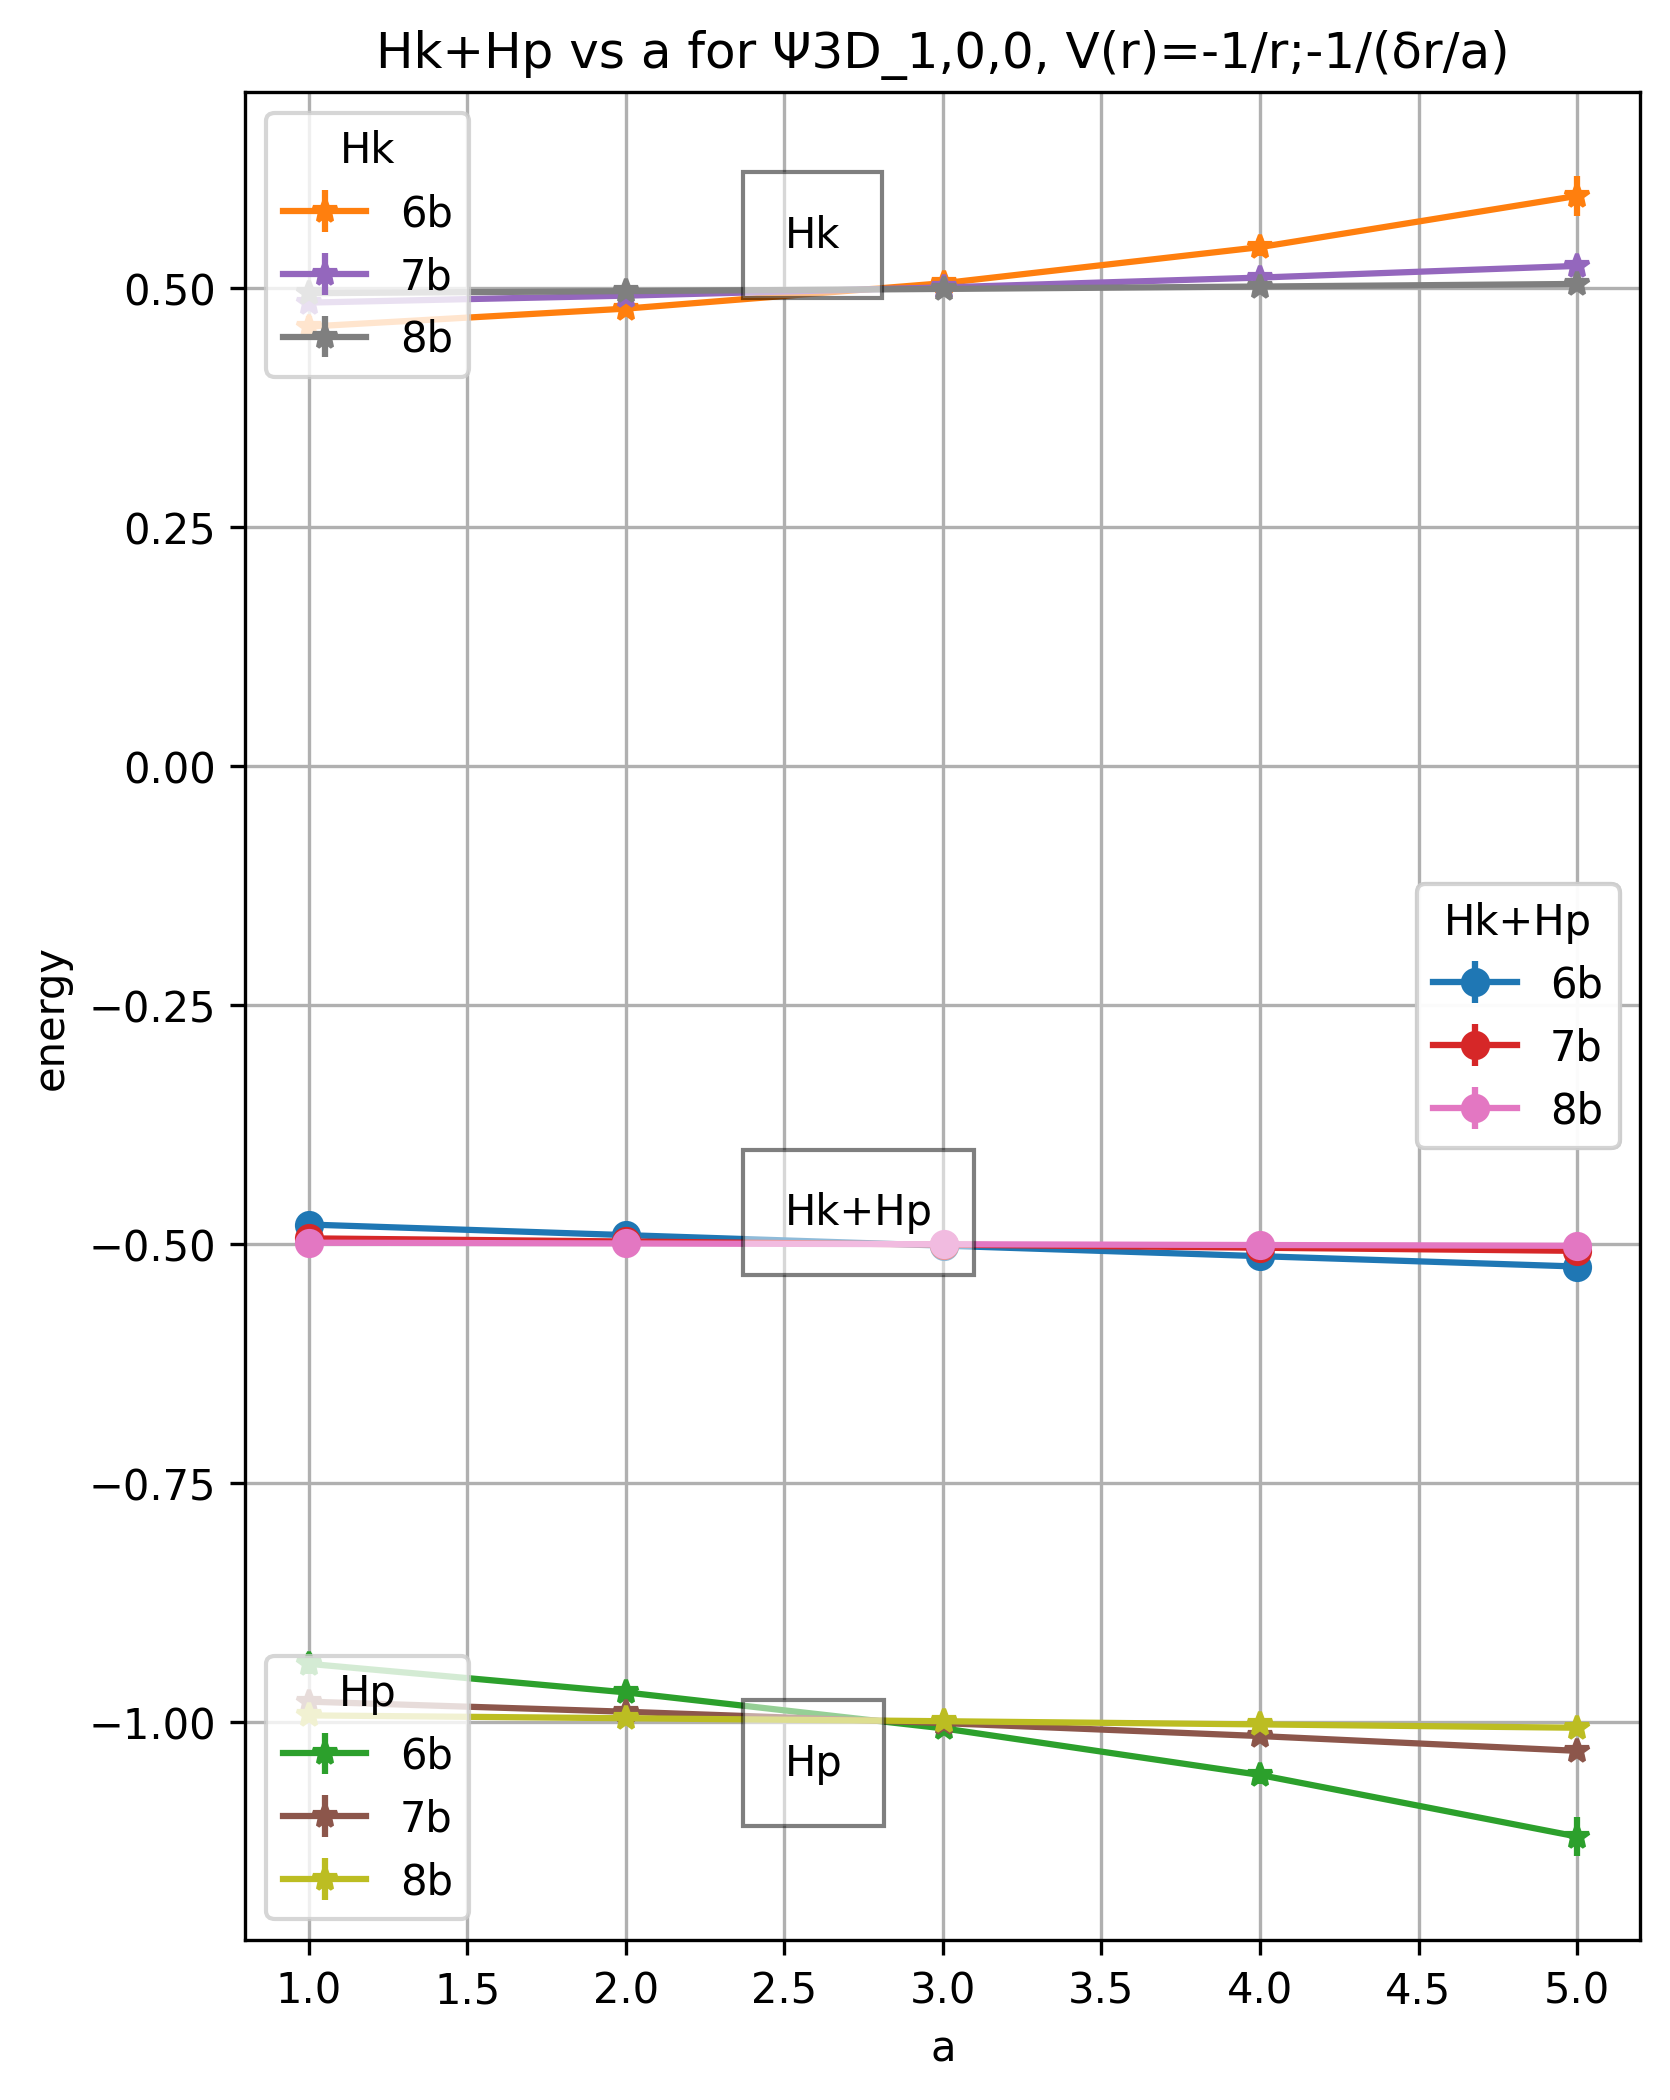
\includegraphics[width=1\columnwidth]{paper2025_figs/compare_energy/compare_energy_h3D_TO2_r0lim_1_0_0.png}
    \caption{Changes in energy values when varying $\reff$ in the approximated formula $\Hla(r)$ for the 3D hydrogen atom model}
    \label{fig:Ha1-vs-delta1-3d}
    \begin{flushleft}\small
      
        Graph for the state $\PsiThreeD_{1,0,0}$, setting $\reff=\deltar/a$ and
        varying $a$. The time evolution period $t=12.6\approx 2\pi/|E_1|$.
        Across all bit counts, the expectation value of the Hamiltonian
        $\Hk+\Hp$ shows a value close to the analytical solution of $-0.5$ a.u. when
        $a=3$ ($\reff=\deltar/3$).
    \end{flushleft}
\end{figure}

\section{Error Evaluation for a Longer Period}
\label{sec:appendix_error_evaluation_t30}
Error evaluation for an extended time evolution period of $t=30$ a.u. is shown in Figs.\ref{fig:trotter-error-t30-part1} and
\ref{fig:trotter-error-t30-part2}.

\begin{figure*}[ht]
    \centering
    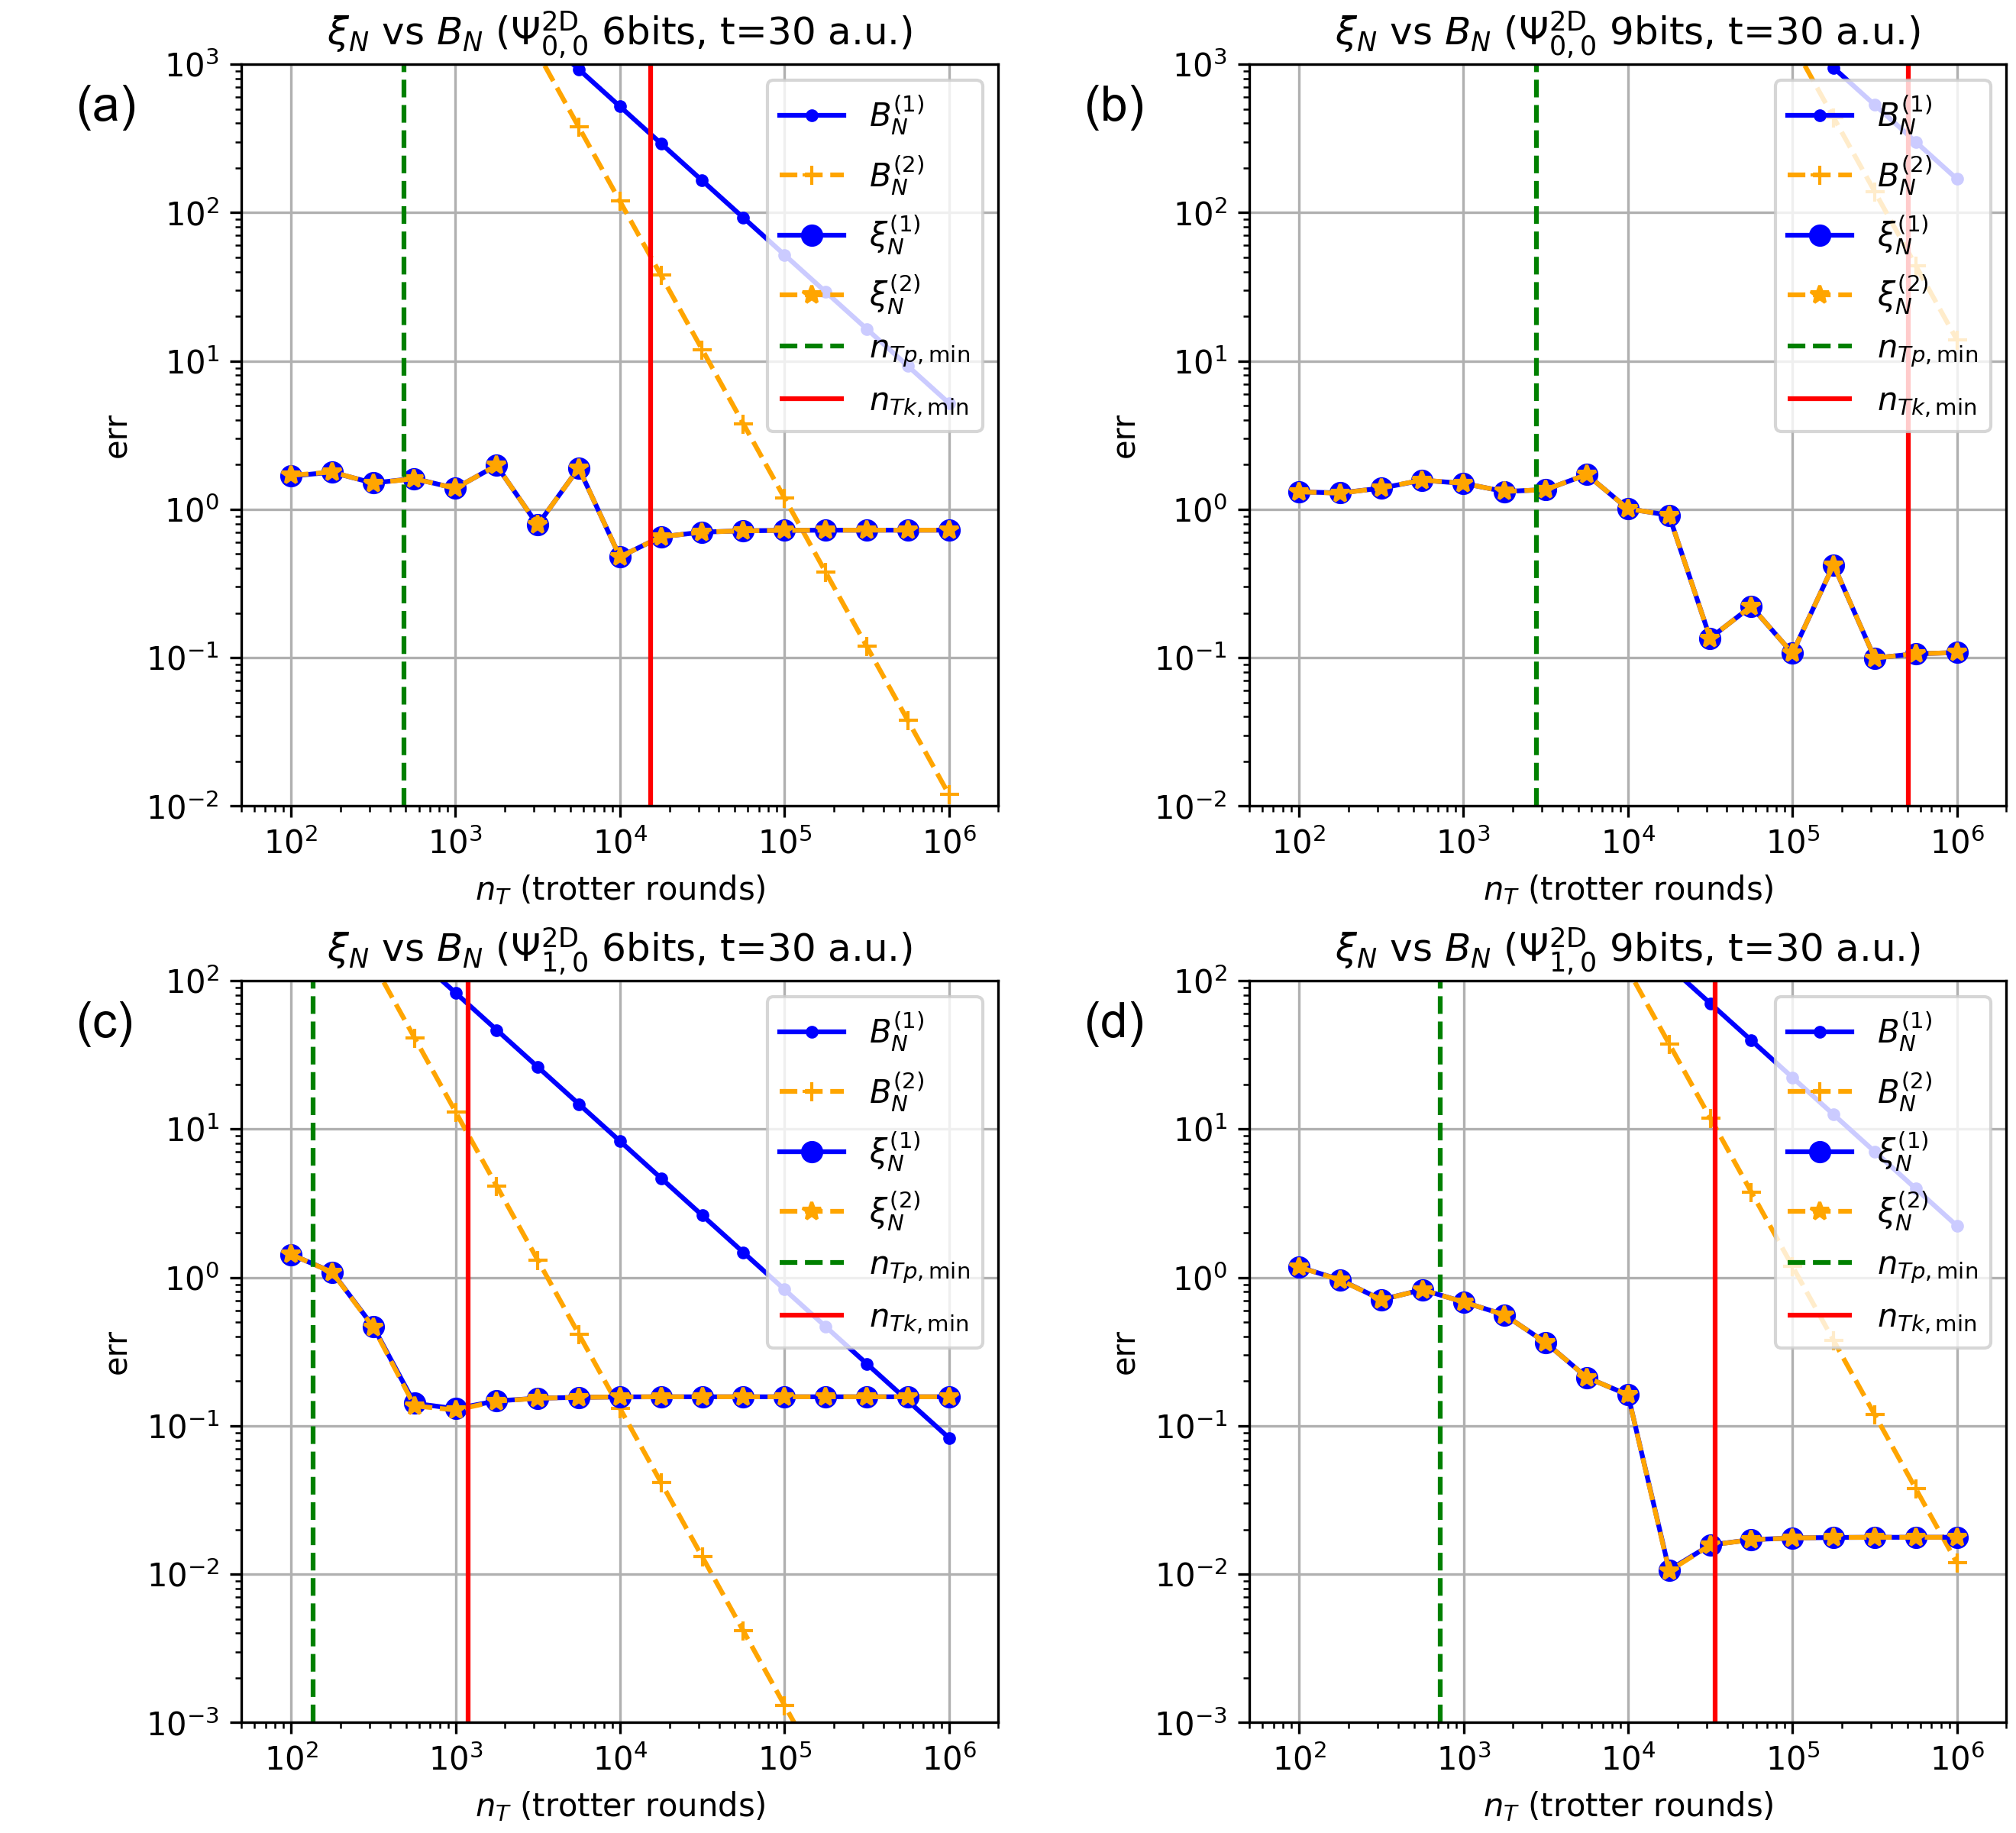
\includegraphics[width=0.8\textwidth]{paper2025_figs/sdt_error/trotter_err_00_10_t30.png}

    \caption{Upper bound $\BN{\gamma}$ and observed value $\xiN{\gamma}$ of the error with respect to the number of divisions $\nT$ at time evolution period $t=30.0$}
    \label{fig:trotter-error-t30-part1}
    \begin{flushleft}\small

        Relationship between the number of Trotter divisions and error in the 2D
        model. The time evolution period is fixed at $t=30.0$.
    
    \end{flushleft}
\end{figure*}

\begin{figure*}[ht]
    \centering
    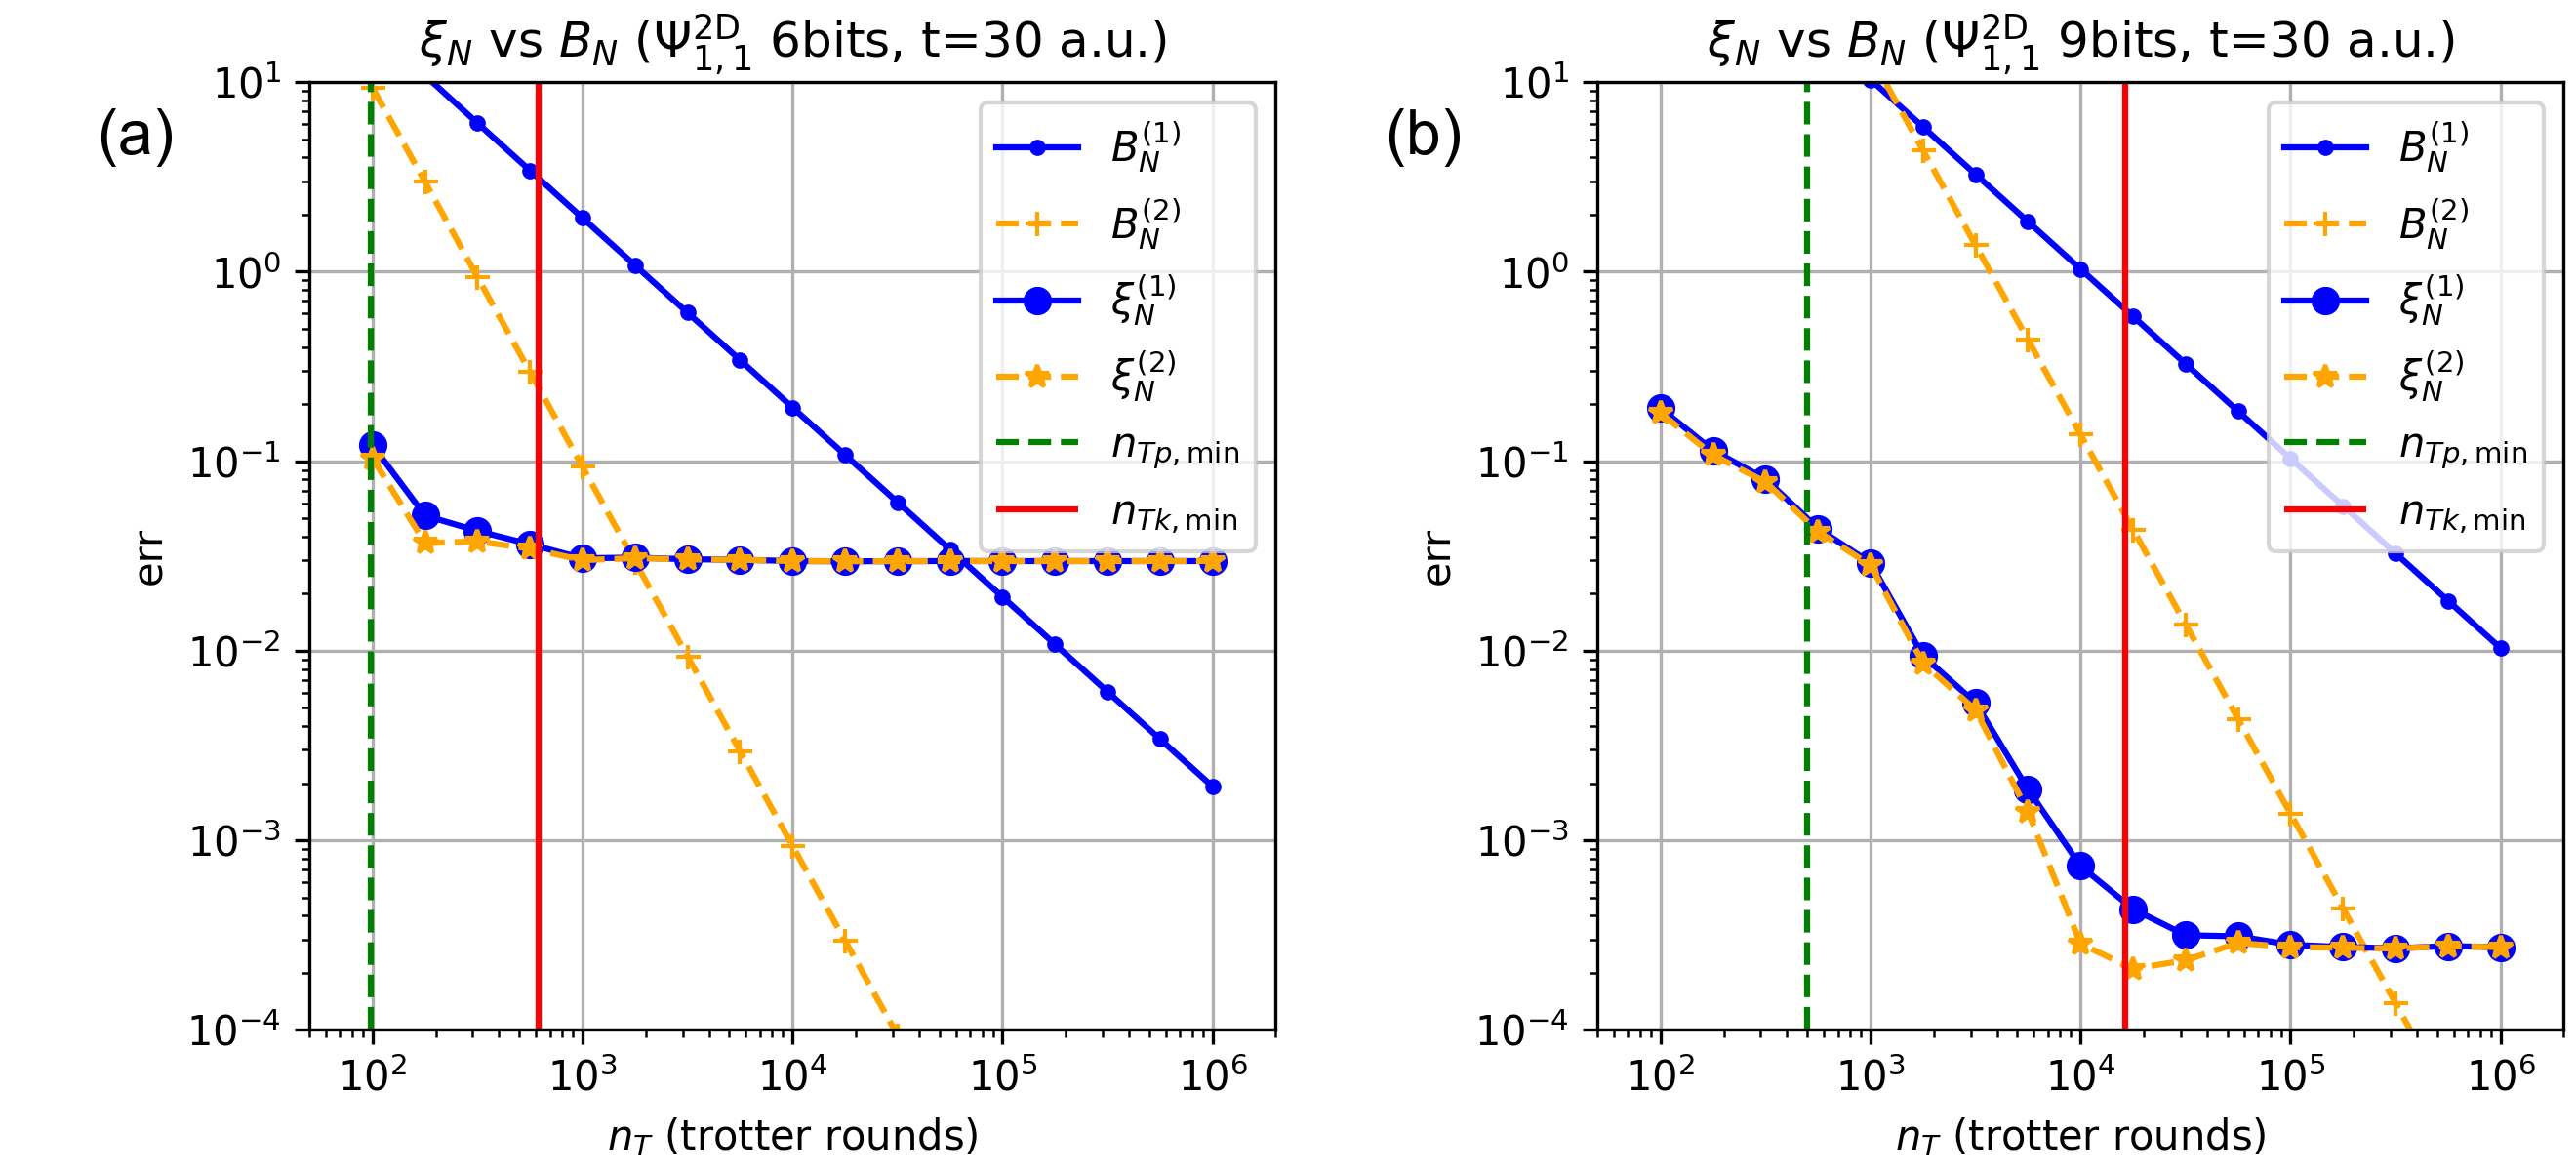
\includegraphics[width=0.8\textwidth]{paper2025_figs/sdt_error/trotter_err_11_t30.png}
    \caption{Upper bound $\BN{\gamma}$ and observed value $\xiN{\gamma}$ of the
    error with respect to the number of divisions $\nT$ at time evolution period
    $t=30.0$ (continued)}
    \label{fig:trotter-error-t30-part2}
    \begin{flushleft}\small

        Evaluation results for the wavefunction $\PsiTwoD_{1,1}$ with azimuthal
        quantum number $m=1$.
    \end{flushleft}
\end{figure*}

%% Only run the bibliography when this subfile is compiled standalone; when
%% \subfile'd into aip-draft.tex, the master's own \bibliography{quantum}
%% (called once, at the very end) handles it instead. Without this guard,
%% REVTeX's automatic end-of-document bibliography hook fires twice (once
%% from revtex4-2.cls, once from the aip4-2 substyle) whenever no explicit
%% \bibliography command is present, producing a duplicate \bibdata entry
%% that bibtex rejects with "Illegal, another \bibdata command".
\ifSubfilesClassLoaded{\bibliography{quantum}}{}

\end{document}
